\documentclass[letterpaper]{article}
\usepackage{aaai24}
\usepackage{times}
\usepackage{helvet}
\usepackage{courier}
\usepackage[hyphens]{url}
\usepackage{graphicx}
\graphicspath{{figures/}}
\urlstyle{rm}
\usepackage{amsmath}
\usepackage{amssymb}
\usepackage{booktabs}
\usepackage{algorithm}
\usepackage{algorithmic}
\usepackage{natbib}
\usepackage{float}

\frenchspacing
\setlength{\pdfpagewidth}{8.5in}
\setlength{\pdfpageheight}{11in}

\title{Q-Learning and Deep Q-Networks for Autonomous Parking Navigation}
\author{
    Josh Manchester\\
    Department of Computer Science\\
    University of Colorado Colorado Springs\\
    Colorado Springs, CO 80918\\
    \texttt{jmanches@uccs.edu}
}

\begin{document}
\maketitle

\begin{abstract}
This paper describes the implementation and evaluation of four reinforcement learning algorithms for a parking lot navigation task: tabular Q-learning, Double Q-learning, Deep Q-Networks (DQN), and DreamerV3. The three model-free methods were built from scratch without RL libraries. A goal-conditioned agent learns to navigate a $7 \times 6$ grid from an entrance to any of 8 parking spots, where non-target spots act as barriers. All model-free algorithms achieve 100\% success rates with BFS-optimal paths. DreamerV3, a model-based method that learns from image observations, achieves near-optimal peak performance but exhibits unstable convergence. The paper covers design decisions, results, and problems encountered during development---including DQN convergence difficulties, state representation design, scaling to a $10 \times 12$ grid, and model-based versus model-free tradeoffs.
\end{abstract}

\section{What Was Done}

Three reinforcement learning algorithms were implemented in Python using only NumPy (for tabular methods) and PyTorch (for DQN). No RL libraries were used.

\subsection{Environment}

The parking lot is a $7 \times 6$ grid (7 rows, 6 columns) with 8 parking spots in two rows (P1--P4 in row 2, P5--P8 in row 4), separated by a barrier on row 3 (columns 1--4). The entrance is at position $(6, 5)$. Columns 0 and 5 on the barrier row are open, providing passages on both sides. Figure~\ref{fig:env} shows the layout.

\begin{figure}[H]
    \centering
    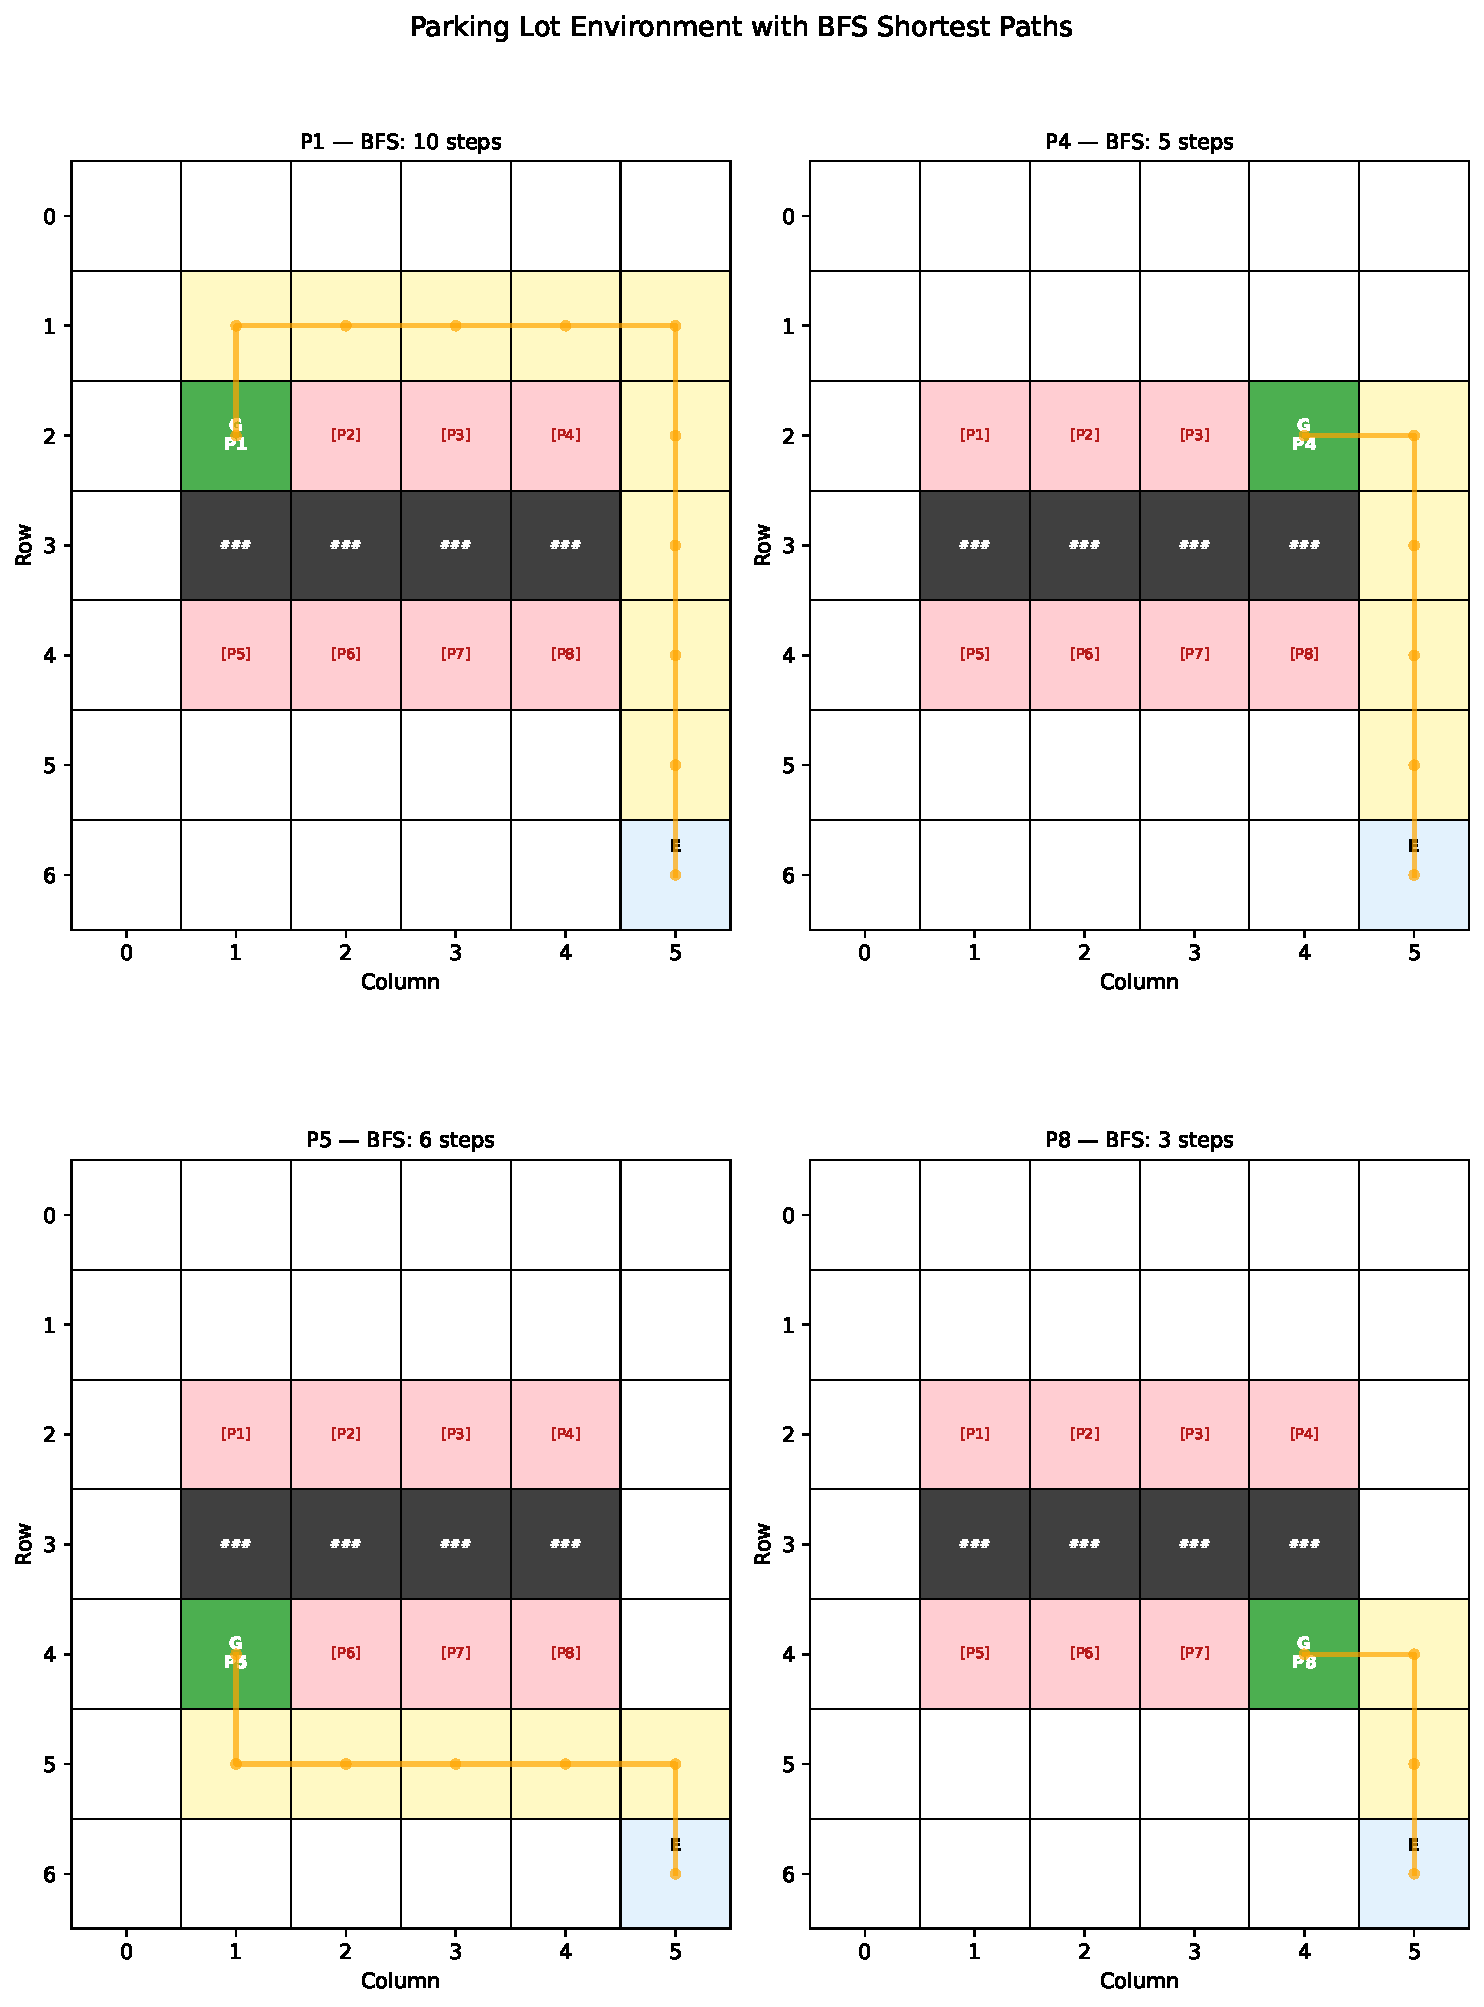
\includegraphics[width=0.95\columnwidth]{environment_layout.pdf}
    \caption{Parking lot with BFS shortest paths for P1 (10 steps), P4 (5 steps), P5 (6 steps), and P8 (3 steps). Green = goal, pink = blocked spots, gray = barrier.}
    \label{fig:env}
\end{figure}

The environment is \textit{goal-conditioned}: the state includes which parking spot the agent is targeting, because non-target spots act as walls. This means each of the 8 goals creates a different navigation problem with its own walkable cells. BFS verification runs at startup to confirm all spots are reachable.

The reward structure uses $+10$ for reaching the goal (terminal), $-0.1$ per step, and $-1.0$ for hitting walls, barriers, or edges. The step penalty encourages shortest paths while the wall penalty discourages bumping into obstacles.

\subsection{Tabular Q-Learning and Double Q-Learning}

Both algorithms use $\varepsilon$-greedy exploration with $\varepsilon$ decaying from 1.0 to 0.01 (factor 0.995 per episode). The Q-table is a Python dictionary mapping $(r, c, g, a) \to \mathbb{R}$, initialized to 0. Hyperparameters: $\alpha = 0.1$, $\gamma = 0.99$.

Q-learning updates use the standard off-policy rule:
\begin{equation}
    Q(S,A) \leftarrow Q(S,A) + \alpha\left[R + \gamma \max_{a'} Q(S',a') - Q(S,A)\right]
\end{equation}

Double Q-learning maintains two tables $Q_1, Q_2$ and randomly updates one using the other for evaluation. This decouples action selection from value estimation, reducing the maximization bias inherent in standard Q-learning \citep{hasselt2010double}.

\subsection{Deep Q-Network}

DQN approximates the Q-function with a neural network: Input(4) $\to$ FC(128) $\to$ ReLU $\to$ FC(128) $\to$ ReLU $\to$ FC(4). The 4-dimensional input encodes the car position and goal position, all normalized to $[0,1]$. The output is Q-values for each of the 4 actions.

Two stabilization mechanisms were used following \citet{mnih2015human}: (1) a replay buffer of 20,000 transitions sampled in mini-batches of 64, and (2) a target network updated every 50 episodes. Training used Adam with learning rate $5 \times 10^{-4}$ and $\varepsilon$-greedy exploration with decay factor 0.998.


\section{Results}

\subsection{Base Grid Performance}

All three algorithms achieve 100\% success across all 8 parking spots, with path lengths matching BFS exactly. Table~\ref{tab:results} shows the evaluation results (identical for all three methods).

\begin{table}[H]
\centering
\caption{Evaluation results (100 episodes per goal)}
\label{tab:results}
\begin{tabular}{@{}ccccc@{}}
\toprule
Spot & Success & Avg Steps & Avg Reward & BFS \\
\midrule
P1 & 100\% & 10.0 & 9.10 & 10 \\
P2 & 100\% & 9.0  & 9.20 & 9 \\
P3 & 100\% & 8.0  & 9.30 & 8 \\
P4 & 100\% & 5.0  & 9.60 & 5 \\
P5 & 100\% & 6.0  & 9.50 & 6 \\
P6 & 100\% & 5.0  & 9.60 & 5 \\
P7 & 100\% & 4.0  & 9.70 & 4 \\
P8 & 100\% & 3.0  & 9.80 & 3 \\
\bottomrule
\end{tabular}
\end{table}

Figure~\ref{fig:qpolicies} shows the Q-learning policies for all 8 goals. The arrows consistently follow the shortest paths.

\begin{figure}[H]
    \centering
    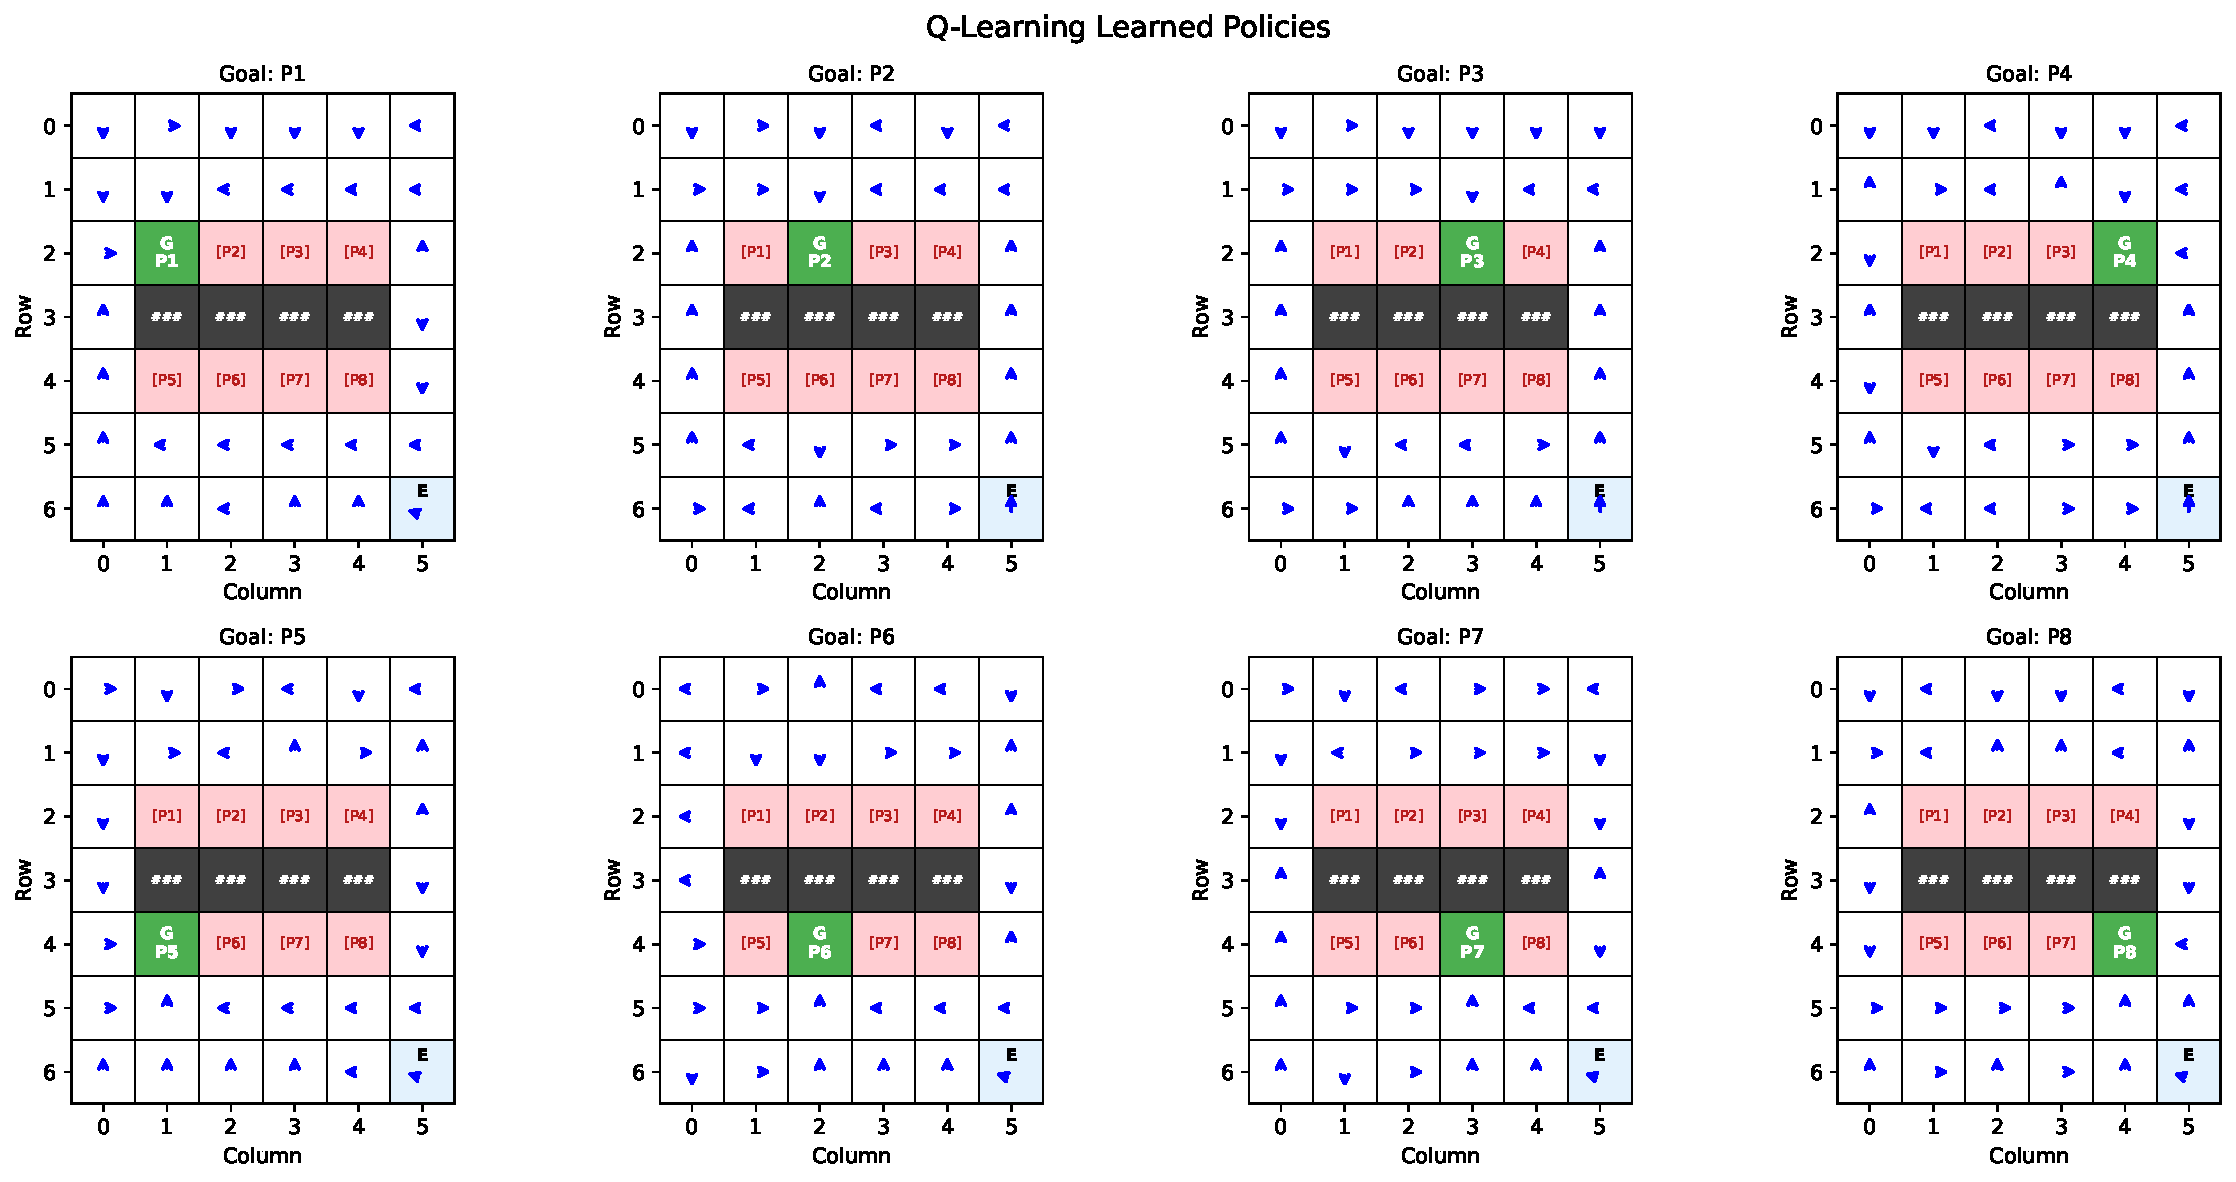
\includegraphics[width=0.95\columnwidth]{q_learning_policies.pdf}
    \caption{Q-learning policies for all 8 spots. Blue arrows show greedy actions.}
    \label{fig:qpolicies}
\end{figure}

\subsection{Convergence}

Q-learning converges in approximately 1,500 episodes, Double Q-learning in approximately 2,000, and DQN in approximately 6,000. Figure~\ref{fig:convergence} compares Q-learning and DQN directly. The tabular methods have a clear advantage on this small grid---there are only $\sim$29 walkable states per goal, well within tabular capacity.

\begin{figure}[H]
    \centering
    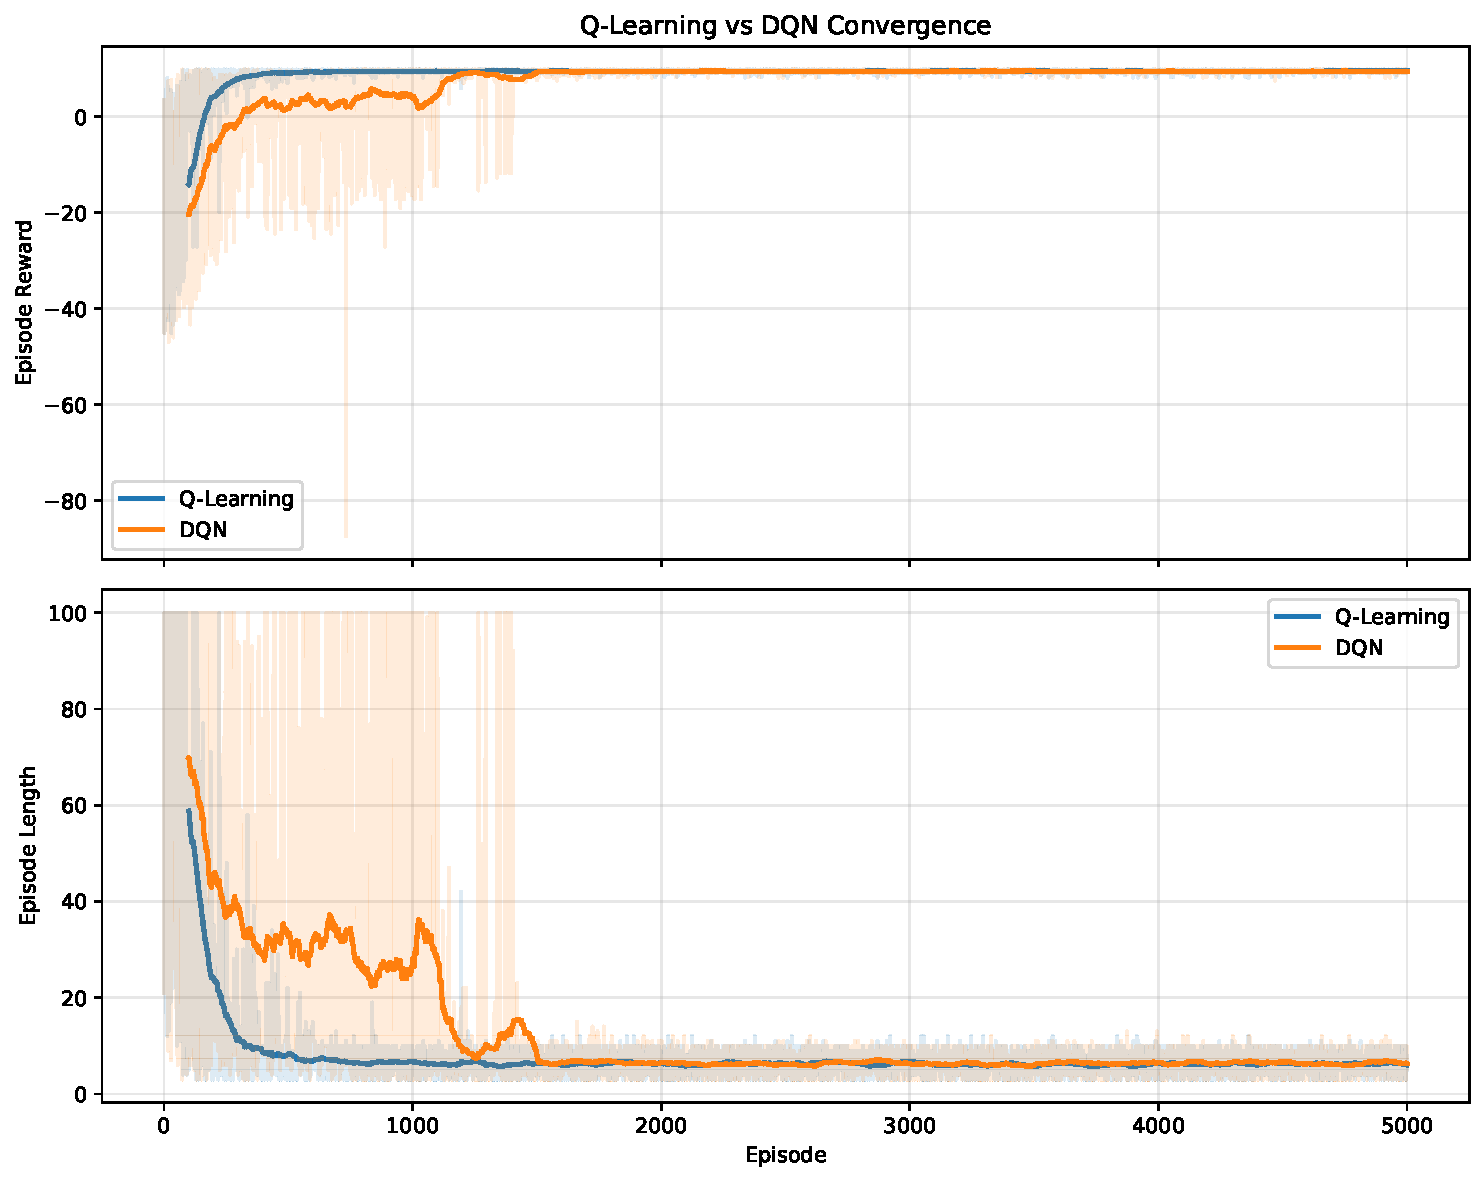
\includegraphics[width=0.95\columnwidth]{dqn_vs_tabular.pdf}
    \caption{Q-learning converges faster than DQN on the $7 \times 6$ grid. Moving average over 100 episodes.}
    \label{fig:convergence}
\end{figure}

\subsection{Overestimation Bias}

Figure~\ref{fig:overest} shows the maximization bias effect. Standard Q-learning's mean max Q-values are consistently higher than Double Q-learning's throughout training. In our deterministic environment this does not hurt final performance, but in stochastic settings it can cause the agent to favor overestimated actions.

\begin{figure}[H]
    \centering
    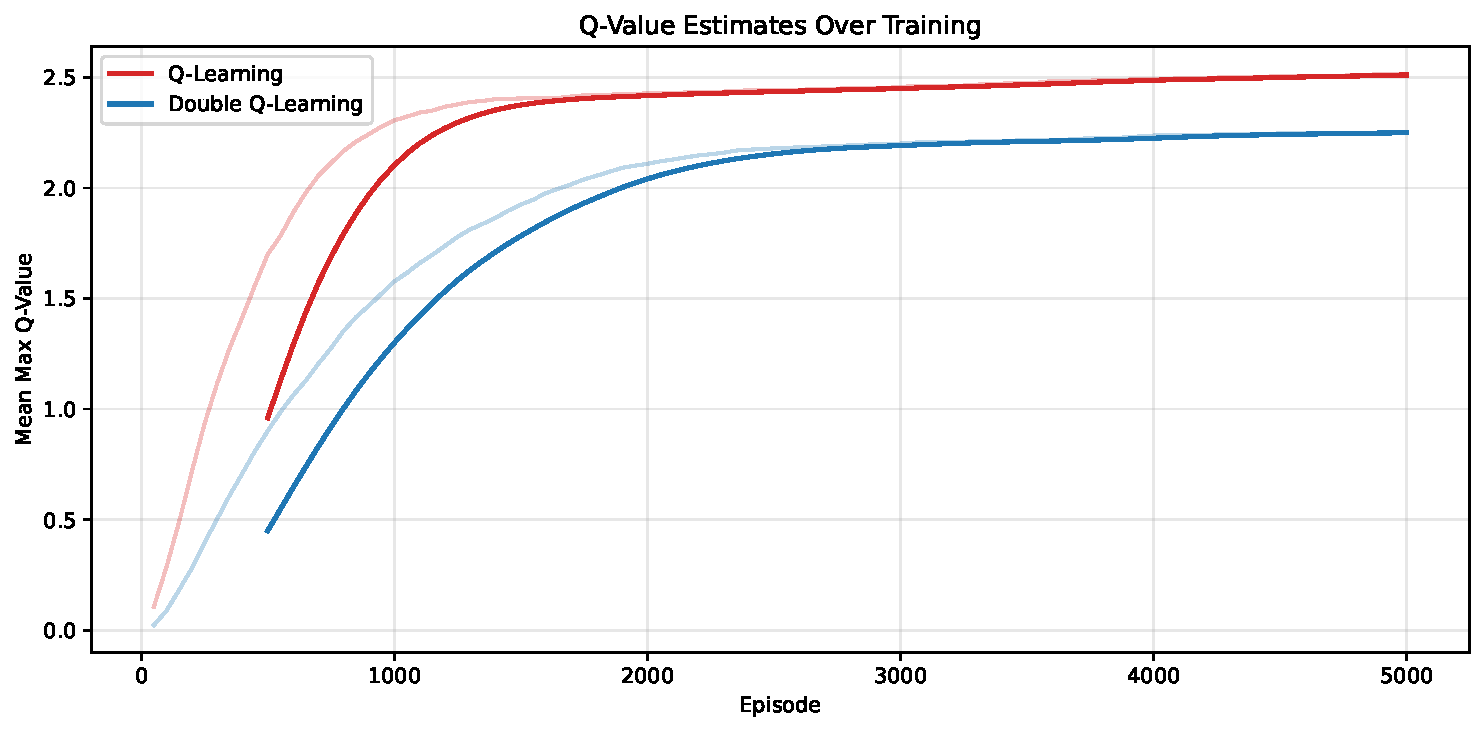
\includegraphics[width=0.95\columnwidth]{q_overestimation.pdf}
    \caption{Q-learning overestimates Q-values compared to Double Q-learning.}
    \label{fig:overest}
\end{figure}

\subsection{Parameter Sensitivity}

Figure~\ref{fig:params} shows Q-learning sensitivity to three parameters. The key finding: $\alpha = 0.1$, $\gamma = 0.99$, and $\varepsilon_{\text{decay}} = 0.995$ are robust defaults. Extreme values ($\alpha = 0.01$ or $\varepsilon_{\text{decay}} = 0.999$) slow convergence but still reach optimality. The algorithm is fairly forgiving across the tested ranges.

\begin{figure}[H]
    \centering
    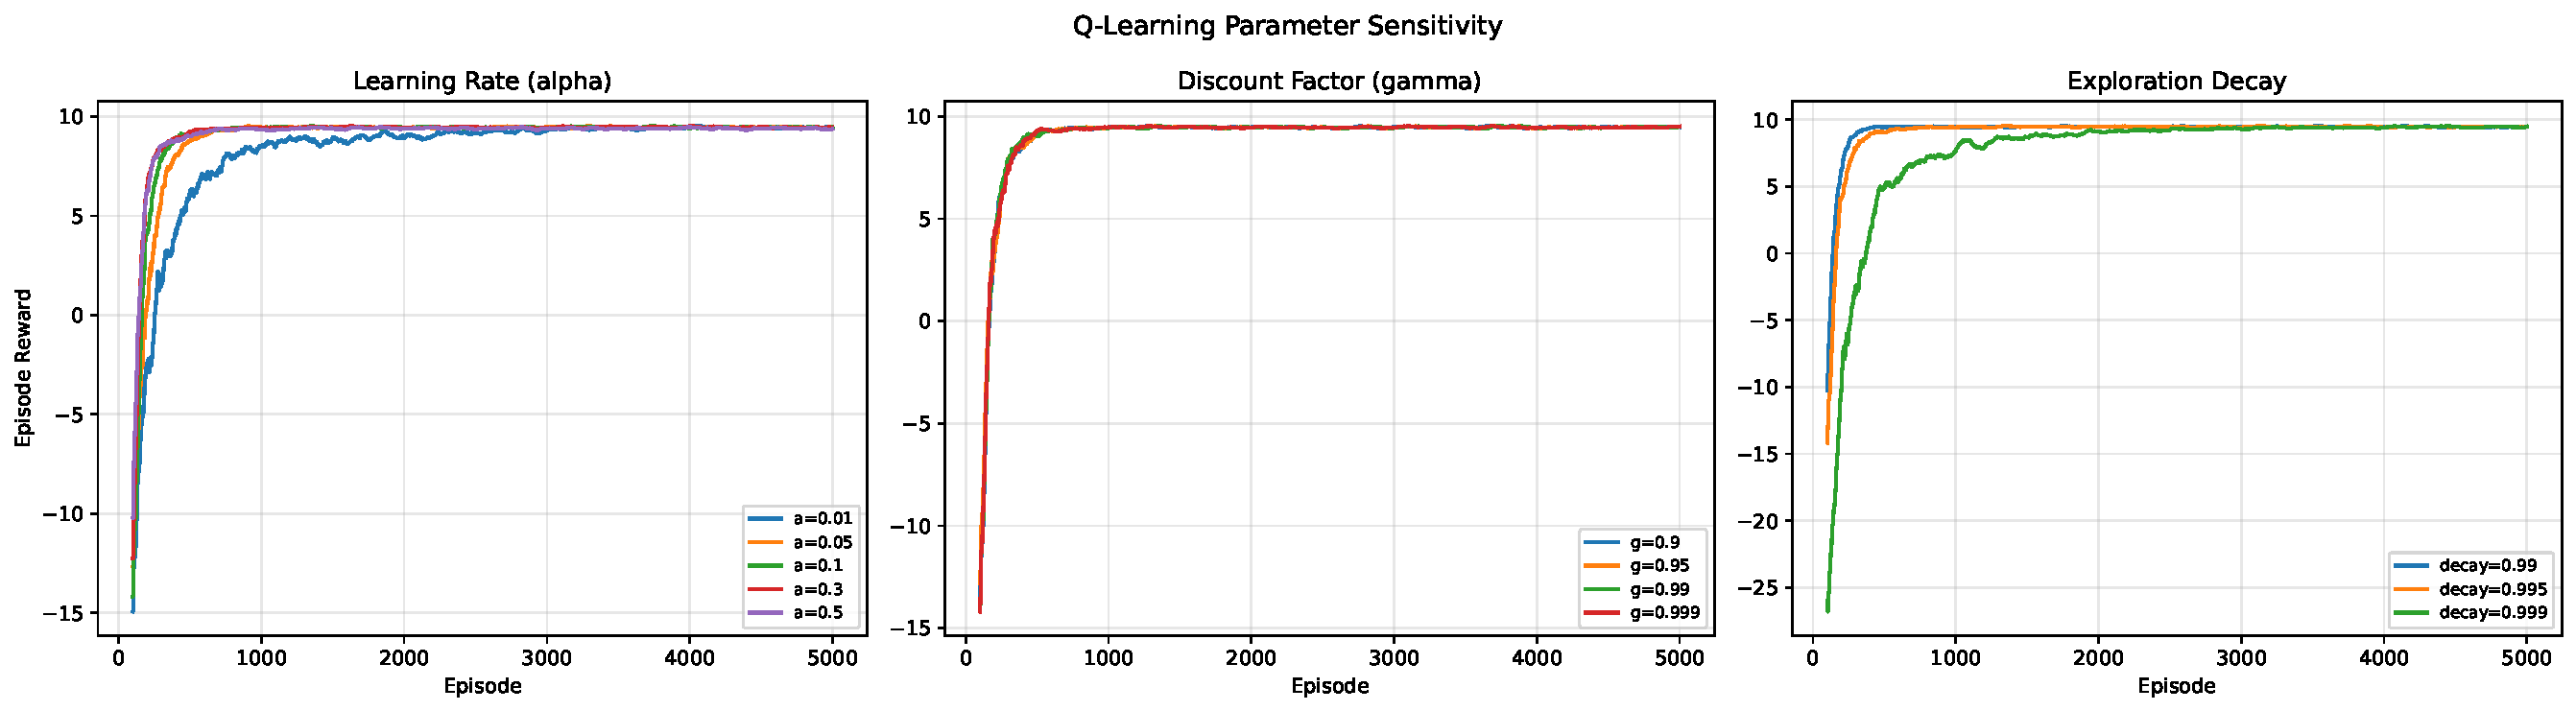
\includegraphics[width=0.95\columnwidth]{tabular_param_sensitivity.pdf}
    \caption{Q-learning parameter sensitivity. Left: learning rate. Center: discount factor. Right: exploration decay.}
    \label{fig:params}
\end{figure}

\subsection{Scaling to $10 \times 12$}

As an enhancement, the environment was extended to a $10 \times 12$ grid with 32 parking spots (generated procedurally using the same layout pattern). All three algorithms achieve 100\% success on the larger grid with BFS-optimal paths (average 11.4 steps vs. 6.3 on the base grid). Episode counts were scaled proportionally with state-space size. DQN required no architecture changes---the same 17,540-parameter network handles both grids because it generalizes from normalized position inputs.


\section{Problems and Solutions}

\subsection{Goal-Conditioned State Design}

The most consequential design decision was making the state goal-conditioned. Initially, the agent was trained without goal information, which meant it learned a single policy for all goals. This does not work because the walkable cells change per goal---a cell occupied by parking spot P3 is blocked when targeting P1, but walkable when targeting P3.

The solution was to include the goal ID in the state for tabular methods (extending the key to $(r, c, g, a)$) and to include the goal position as neural network input for DQN. This multiplies the effective state space by 8 but correctly captures that navigation to P1 is a fundamentally different problem than navigation to P8.

\subsection{DQN Convergence}

DQN initially used 64-unit hidden layers and converged inconsistently---some goals (particularly P1, the farthest spot) failed entirely at 3,000 training episodes. Two changes fixed this:

\begin{enumerate}
    \item Increasing hidden layer width from 64 to 128 units. The 64-unit network lacked capacity to represent 8 distinct goal-conditioned policies simultaneously.
    \item Slowing $\varepsilon$ decay from 0.995 to 0.998. Neural networks benefit from extended exploration because early Q-value estimates are noisy, and exploiting noisy estimates fills the replay buffer with poor-quality data.
\end{enumerate}

With these changes, DQN reaches 100\% success across all goals within 6,000 episodes.

\subsection{Barrier Routing Asymmetry}

Bottom-row spots (P5--P8) are directly accessible from the entrance in 3--6 steps. Top-row spots (P1--P4) require routing around the barrier, through columns 0 or 5, and back across the top lanes---10 steps for P1. This asymmetry means the agent encounters top-row goals less frequently during exploration (it often times out before reaching them early in training). The decaying exploration schedule helps: early random exploration eventually stumbles onto successful top-row paths, which then get reinforced.

\subsection{Replay Buffer Sizing}

The replay buffer size affects DQN's sample efficiency. Too small (1,000 transitions) and the buffer holds only recent data, causing catastrophic forgetting of earlier goals. Too large (50,000+) and the buffer retains many low-quality transitions from the random exploration phase, slowing convergence. Testing showed 10,000--20,000 to be the effective range. We settled on 20,000, which stores roughly 3,000 episodes of experience at convergence.


\section{DreamerV3: Model-Based Comparison}

DreamerV3 \citep{hafner2023dreamerv3} was also trained on the $7 \times 6$ parking lot to compare a model-based approach against the three model-free methods. DreamerV3 learns a world model from image observations and trains its policy entirely in ``imagination''---dreamed trajectories generated by the learned model---rather than from direct environment interaction.

The parking lot was wrapped as a Gymnasium environment producing $64 \times 64$ RGB images. Each cell type has a distinct color: dark gray for roads, medium gray for barriers, blue for non-goal parking spots, red for the goal spot, amber for the entrance, and green for the agent. The goal spot's color encodes the goal-conditioned information that tabular methods receive as part of the state tuple.

Training ran for 100,000 environment steps with 4 parallel environments, train ratio 512 (dream steps per real step), and a discount of 0.99. Table~\ref{tab:dreamer} shows selected evaluation results.

\begin{table}[H]
\centering
\caption{DreamerV3 evaluation returns over 100K training steps}
\label{tab:dreamer}
\begin{tabular}{@{}cc@{}}
\toprule
Step & Eval Return \\
\midrule
2,500  & $-65.3$ \\
22,500 & $+9.7$ \\
27,500 & $+9.6$ \\
42,500 & $+9.4$ \\
77,500 & $+9.4$ \\
102,500 & $+8.6$ \\
\midrule
\multicolumn{2}{c}{Peak: $+9.7$ (step 22,500)} \\
\multicolumn{2}{c}{Last 5 avg: $+3.9$} \\
\bottomrule
\end{tabular}
\end{table}

DreamerV3 learns the task quickly---by step 22,500, peak eval return reaches 9.7 (near-optimal, corresponding to $\sim$4 steps on a nearby goal). However, performance is unstable. Returns oscillate between near-optimal runs (9.4--9.7, with 4--7 step paths) and poor runs (1.5--5.7, with 23--100 step paths). The last 5 evaluations average only 3.9, far below the consistent 9.1--9.8 that all three model-free methods achieve after convergence.

The instability likely stems from the goal-conditioned nature of the task. DreamerV3 must learn 8 different navigation policies from pixel observations alone, with the only distinguishing signal being which cell is red. The tabular methods receive the goal ID directly as part of the state, giving them an unambiguous representation. DreamerV3's world model must first learn to decode the goal from the image, then plan accordingly---a harder representational problem compressed into a small $7 \times 6$ visual space where all goals look similar.

This result highlights that model-based RL is not automatically superior. On small, discrete, deterministic problems, tabular methods converge faster, achieve perfect reliability, and require no GPU. DreamerV3's strengths---sample efficiency through imagination, scalability to continuous control, transfer learning---are unnecessary here. The parking lot is small enough that direct experience is cheap and exhaustive, removing the advantage of learning a world model.


\section{Conclusion}

All three model-free algorithms were implemented from scratch and learn optimal parking navigation policies on the $7 \times 6$ grid. The implementations were verified against BFS ground truth---every learned policy matches the shortest path exactly. DreamerV3 demonstrates that a model-based approach can learn the task from raw pixels, but its unstable convergence on this small problem shows that world models are better suited to environments where direct experience is expensive or the state space is too large for tabular methods. The key takeaway is that algorithm choice should match the problem: tabular methods dominate small discrete tasks, DQN scales to larger grids without growing memory, and model-based methods earn their complexity only when imagination is cheaper than real interaction.

\bibliography{references}

\end{document}
